\section{Formulating Recursive Cases}

\begin{Def}[Dynamic Programming]

In recursive algorithms, there are many cases where we repeat
the same computations multiple times. To reduce this redundancy, we store
the results of these computations in a table. This is known as \textbf{memoization}. This paradigm of programming is
called \textbf{dynamic programming}.
\end{Def}
\textbf{Scenario - \textit{Fibonacci Sequence}:} The Fibonacci sequence is defined as $F_n=F_{n-1}+F_{n-2}$, with $F_0=0$ and $F_1=1$. Our
first 8 terms are $\{0,1,1,2,3,5,8,13\}$. To compute $F_5$, we do $0+1=1$, $1+1=2$, $1+2=3$, and $2+3=5$.\\

\noindent
A recursive approach would be:

\begin{Func}[Slow Fibonacci Sequence - \textit{Fib()}]
    \noindent
    \textbf{Input:} $n$ the index of the Fibonacci sequence we wish to compute.\\
    \textbf{Output:} $F_n$ the $n_{th}$ Fibonacci number.\\

    \vspace{-.5em}
    \begin{algorithm}[H]
        \SetAlgoLined
        \SetKwProg{Fn}{Function}{:}{\KwRet{}}
        \Fn{\textit{Fib}($n$)}{
            \If{$n \leq 1$}{
                \textbf{return} $n$\;
            }
            \Else{
                \textbf{return} $\textit{Fib}(n-1)+\textit{Fib}(n-2)$\;
            }
        }
    \end{algorithm}
    \noindent
    \rule{\textwidth}{0.4pt}
    \textbf{Time Complexity:} $O(2^n)$. Since line 6 depends on both calls, we reflect such in our recurrence relation, $T(n)=T(n-1)+T(n-2)+O(1)$, Theorem (\ref{theo:master}). Since we make
    calls of size $n-1$ and $n-2$, which are both $O(n)$, we have an exponential time complexity $O(2^n)$.
\end{Func}

\newpage
\noindent
When we unravel the recursion tree, we see plenty of redundancies:

\begin{figure}[h]


\hspace{5em} 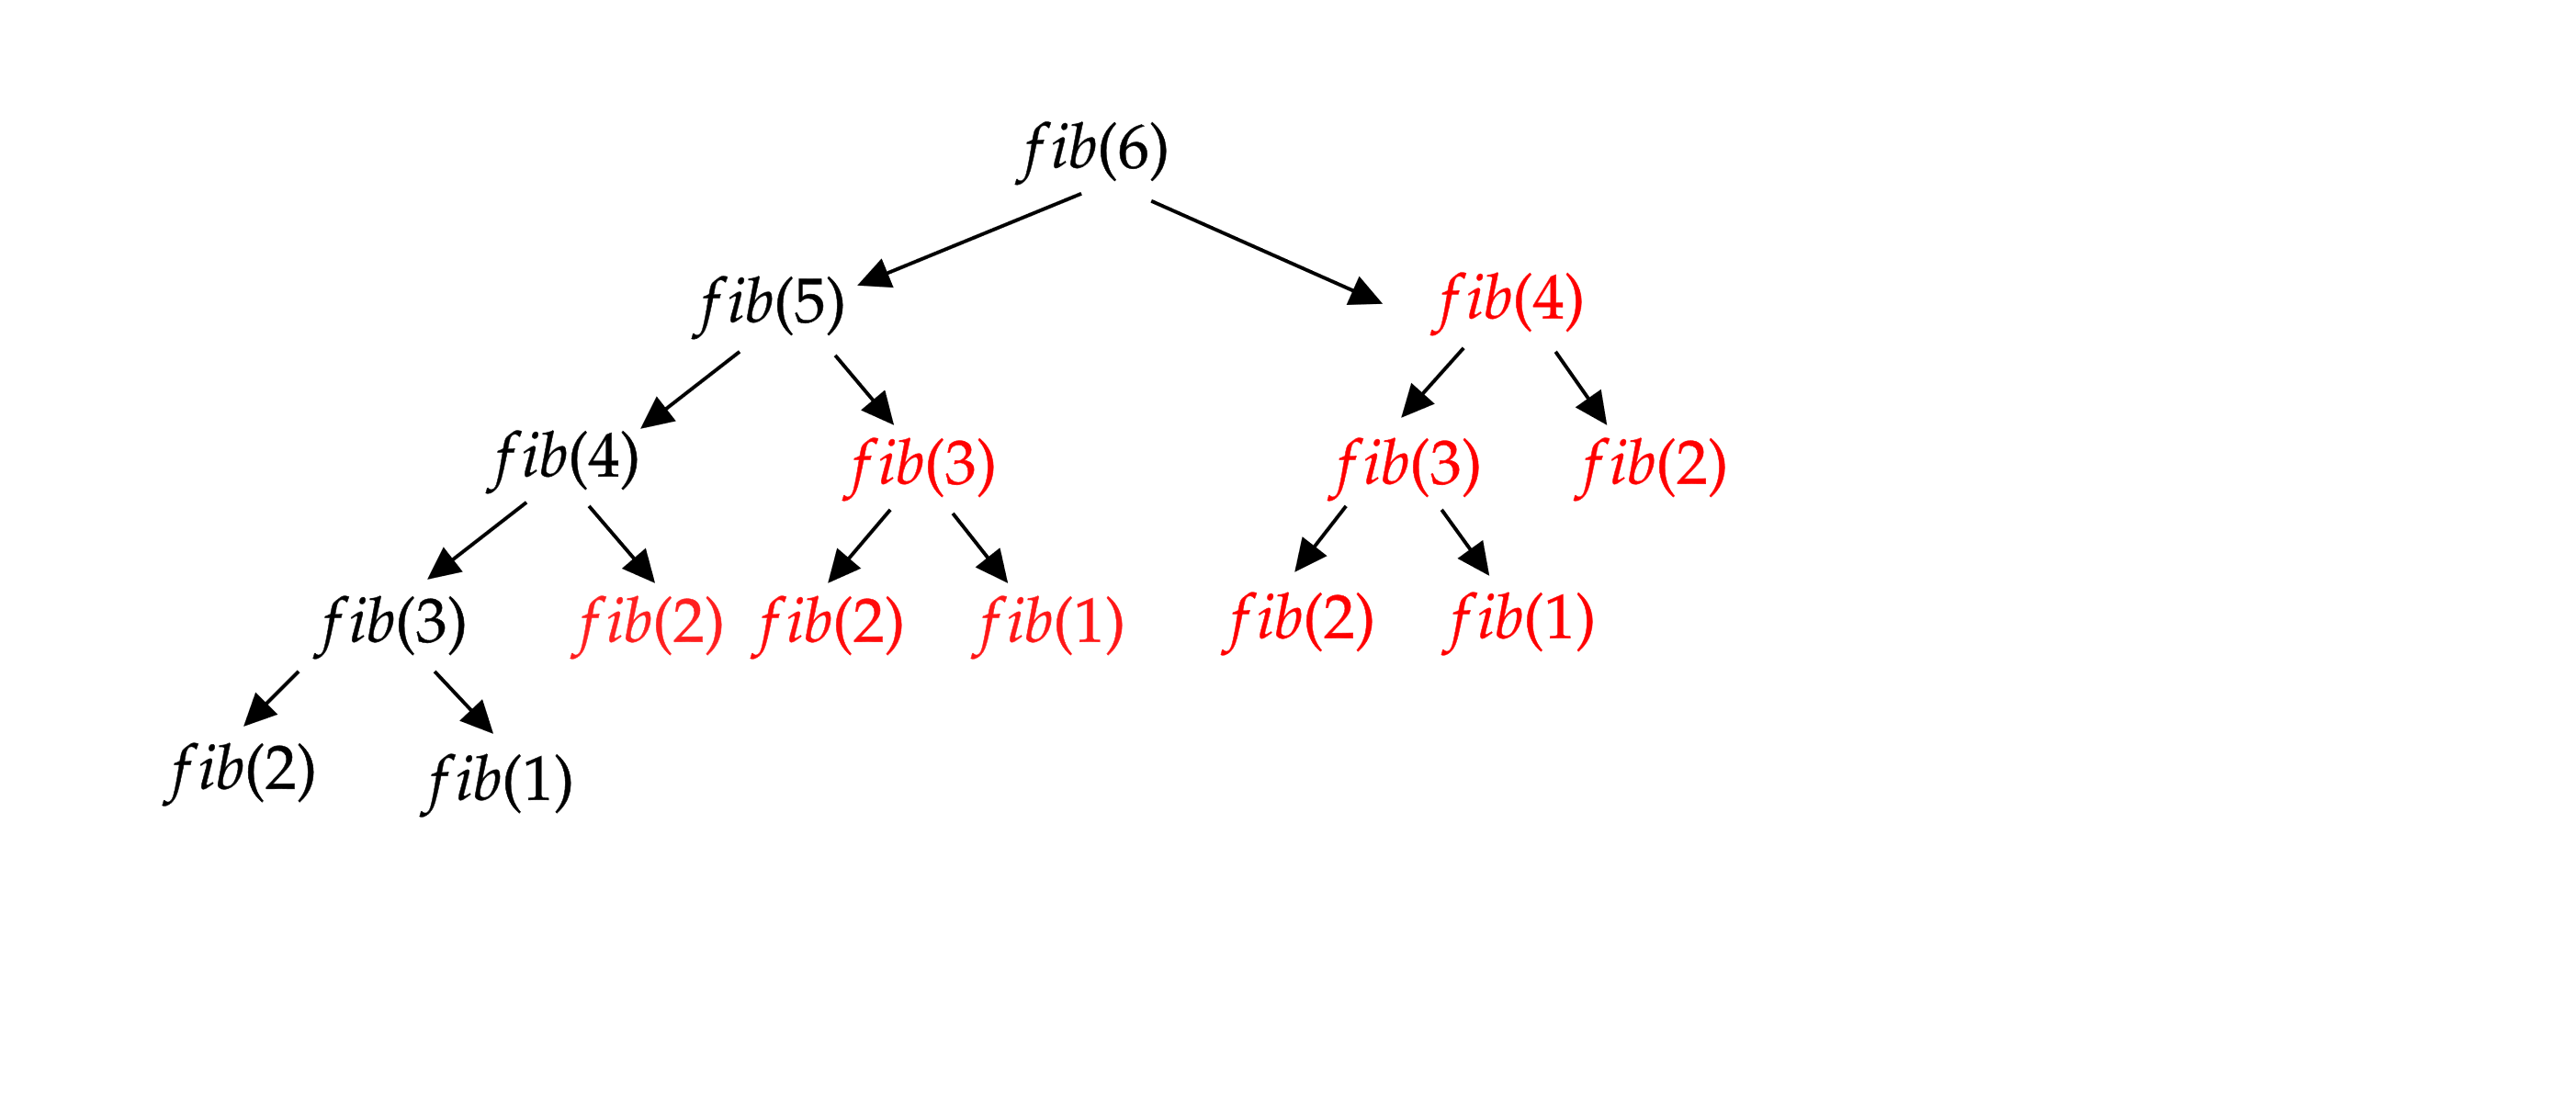
\includegraphics[width=1\textwidth]{Sections/dp/fib.png}

\vspace{-3em}
\caption{Recursion Tree for Fibonacci Sequence}
\label{fig:fib}
\end{figure}

\noindent
We see that we've already computed $F_2$ and $F_3$ multiple times. We can store these values in a table, and use them when needed:

\begin{Func}[Memo Fibonacci Sequence - \textit{Fib()}]

    \textbf{Input:} $n$ the index of the Fibonacci sequence we wish to compute.\\
    \textbf{Output:} $F_n$ the $n_{th}$ Fibonacci number.\\

    \vspace{-.5em}
    \begin{algorithm}[H]
        \SetAlgoLined
        \SetKwProg{Fn}{Function}{:}{\KwRet{}}
        $F[\ ]$; \tcp{Table to store Fibonacci numbers}
        \Fn{\textit{Fib}($n$)}{
            \If{$n \leq 1$}{
                \textbf{return} $n$\;
            }
            \Else{
                \If{$F[n]$ is not defined}{
                    $F[n] = \textit{Fib}(n-1)+\textit{Fib}(n-2)$\;
                }
                \textbf{return} $F[n]$\;
            }
        }
    \end{algorithm}
    \noindent
    \rule{\textwidth}{0.4pt}
    \textbf{Time Complexity:} $O(n)$. Since we only need to compute $F_n$ once, we at most recurse $n-1$ times. As
    we unravel we have all our necessary values stored in our table.\\
    \textbf{Space Complexity:} $O(n)$. We store $n$ and recurse at most $n-1$ times.
\end{Func}


\newpage
\label{sec:WIS}
\noindent
\textbf{Scenario - \textit{Weighted Interval Scheduling}}: Say we have $n$ paying jobs which overlap each other.
We want to find the best set of jobs that allows us to maximize our profit. Recall Section (\ref{sec:interval})

\begin{figure}[h]
\centering
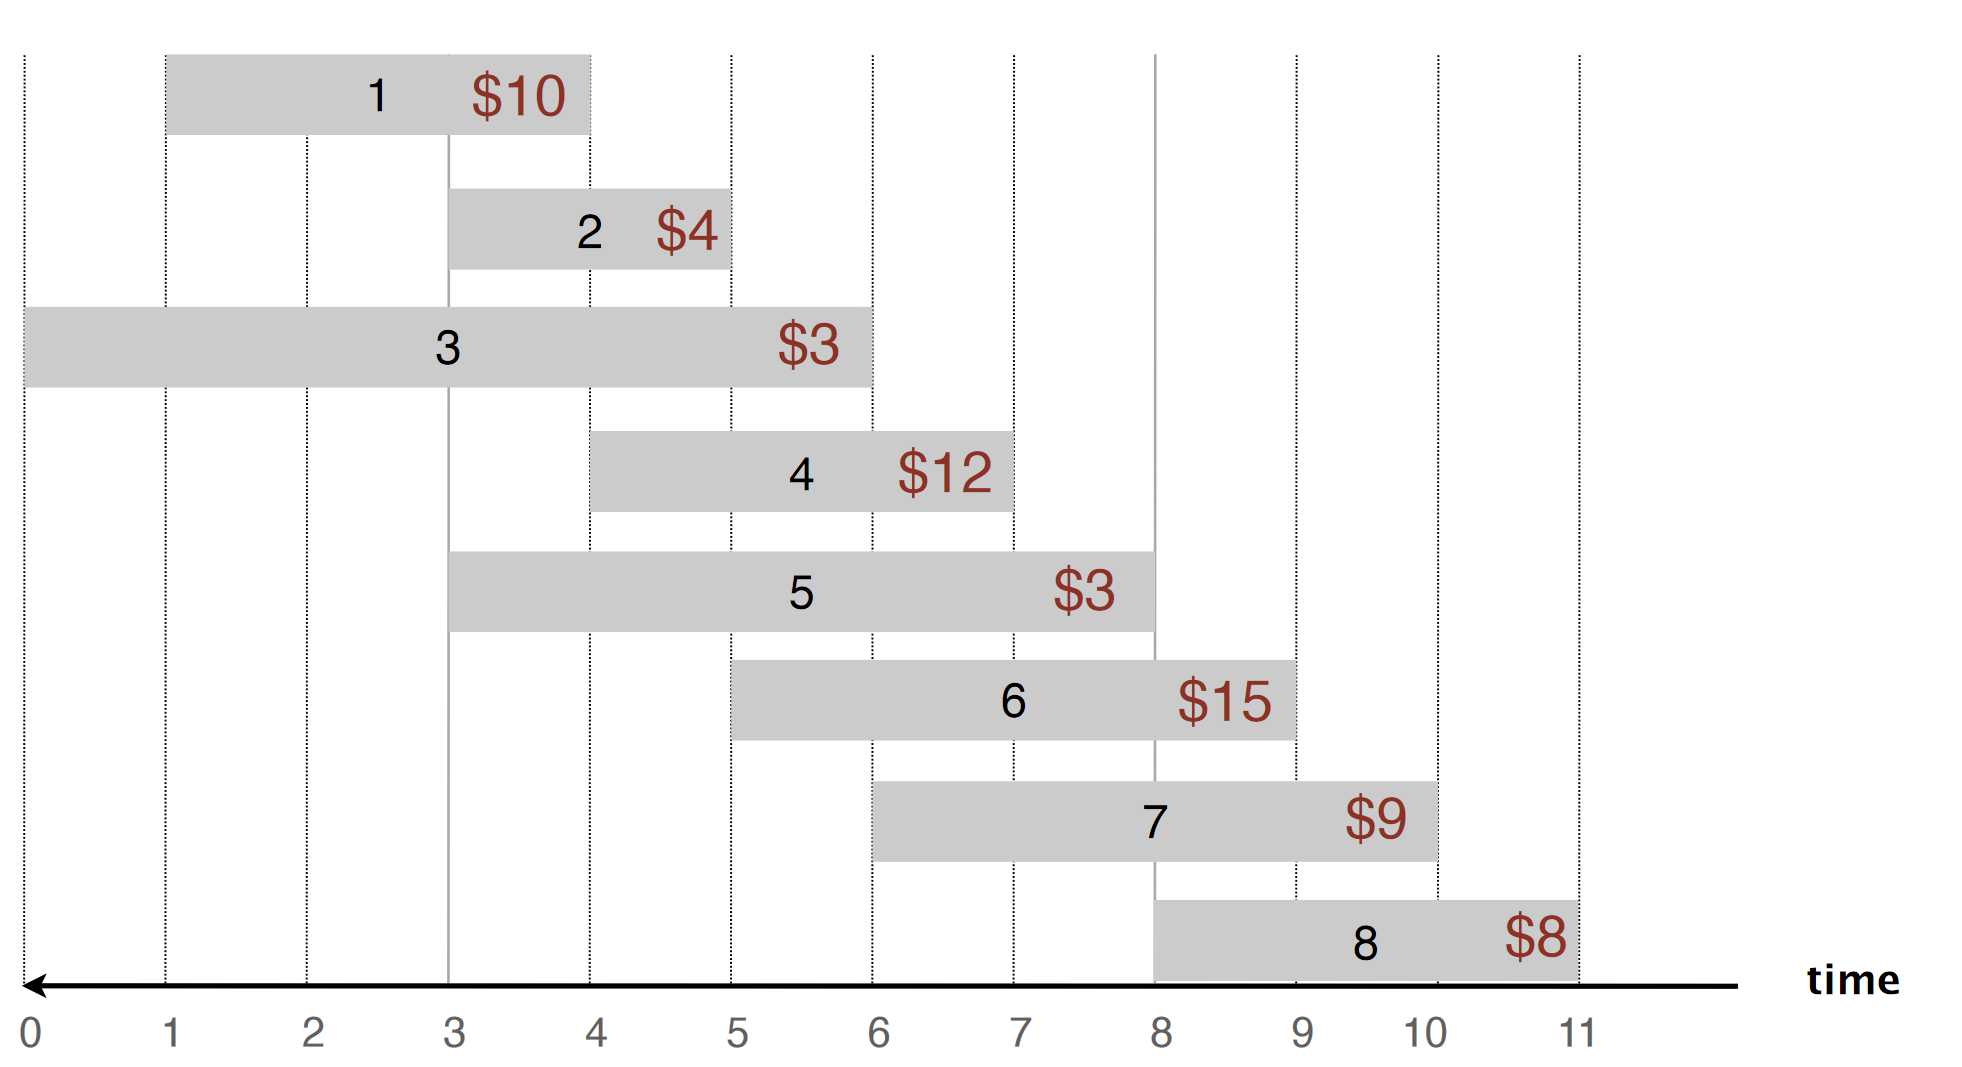
\includegraphics[width=.7\textwidth]{Sections/dp/wis.png}
\end{figure}

\noindent
Let us define $\mathbf{OPT(j)}$ as the maximum profit from jobs $\{1\dots j\}$, and $\mathbf{v_j}$ as $j_{th}$'s value. Then $OTP(8)$, considers jobs $1\dots 8$. Let $p(j):=$ The largest index $i < j$, s.t., job $i$ is compatible with $j$.\\
(if none, then $p(j) = 0$). We have two cases:

\vspace{-1em}
\begin{align*}
    OPT(8) =
    \begin{cases}
        OPT(7) & \text{if job 8 is not selected}\\
        v_8 + OPT(p(8)) & \text{if job 8 is selected}
    \end{cases}
\end{align*}

\noindent
Then $p(8)=5$, $p(5)=0$, yielding $\$11$, which isn't the optimal solution, see job 6.
If we don't choose $j$, then the optimal solution resides in $\{1\dots j-1\}$. So we want to know,
if our current $OPT()$ solution larger than the next solution. We derive the following cases, and algorithm:
\begin{align*}
    OPT(j) =
    \begin{cases}
        0 & \text{if $j=0$}\\
        max\{\underbracket{v_j+OPT(p(j))}_{\text{build solution}}, \underbracket{OPT(j-1)}_{\text{next solution}}\} & \text{else}
    \end{cases}
\end{align*}

\vspace{-1em}
\begin{Func}[Weighted Interval Scheduling - \textit{RecOPT()}]

    \vspace{-.5em}
    Compute all $OPT(j)$ recursivley, unraveling seeing which $OPT(j)$ is larger; $\mathbf{O(2^n)}$ \textbf{Time}.\\
        \begin{algorithm}[H]
            \SetAlgoLined
            \SetKwProg{Fn}{Function}{:}{}
            \Fn{\textit{RecOPT}($j$)}{
                \If{$j = 0$}{
                    \textbf{return} $0$\;
                }
                \Else{
                    $OPT(j) \gets max\{v_j+RecOPT(p(j)), RecOPT(j-1)\}$\;
                    \textbf{return} $OPT(j)$\;
                }
            }
        \end{algorithm}
    \end{Func}

    \newpage

    \noindent
    Now we employ memoization to store our results in a table, and use them when needed:

    \begin{Func}[Memo Weighted Interval Scheduling - \textit{OPT()}]

        \vspace{-.5em}
        \begin{algorithm}[H]
            Sort jobs by finish time; \tcp{$O(n\log n)$}
            Compute all $p(1),\dots,p(n)$; \tcp{$O(n)$}
            \SetKwProg{Fn}{Function}{:}{}
            $OPT[\ ]$; \tcp{Table to store $OPT(j)$}
            \Fn{\textit{OPT}($j$)}{
                \If{$j = 0$}{
                    \textbf{return} $0$\;
                }
                \Else{
                    \If{$OPT[j]$ is not defined}{
                        $OPT[j] \gets max\{v_j+OPT(p(j)), OPT(j-1)\}$; \tcp{$O(n)$}
                    }
                    \textbf{return} $OPT[j]$\;
                }
            }
        \end{algorithm}
        \noindent
        \rule{\textwidth}{0.4pt}
        \textbf{Time Complexity:} $O(n\log n)$, as we are bottle-necked by our sorting algorithm. Line 10 is $O(n)$, following
        the same memoization pattern as the Fibonacci sequence.
    \end{Func}

    \vspace{-2em}
    \section{Bottom-Up Dynamic Programming}
    In the fibonacci, sequence we don't have to compute it recursively. As shown before we can compute it linearly. Computing $F_5$, we do $0+1=1$, $1+1=2$, $1+2=3$, and $2+3=5$.

    \begin{Func}[Bottom-Up Fibonacci Sequence - \textit{Fib()}]

        \vspace{-.5em}
        \begin{algorithm}[H]
            \SetAlgoLined
            \SetKwProg{Fn}{Function}{:}{}
            $F[0] \gets 0$; $F[1] \gets 1$; \tcp{Base cases (array of size $n+1$)}
            \For{$i \gets 2$ \KwTo $n$}{
                $F[i] \gets F[i-1]+F[i-2]$\;
            }
            \textbf{return} $F[n]$\;
        \end{algorithm}
        \noindent
        \rule{\textwidth}{0.4pt}
        \textbf{Time Complexity:} $O(n)$. We compute $F_n$ linearly, only needing to compute $F_i$ once.
    \end{Func}
    \noindent
    To offer intuition, recall figure (\ref{fig:fib}), we see that that we only really take one branch of the tree. All other branches are
    redundant. I.e., it's almost as if we have a linear path from the root to the leaf. Hence, there's no need for recursion.

    \newpage
    \noindent
    Likewise, we can compute the weighted interval scheduling problem linearly:
    \begin{Func}[Bottom-Up Weighted Interval Scheduling - \textit{OPT()}]

        \vspace{-.5em}
        \begin{algorithm}[H]
            \SetAlgoLined
            \SetKwProg{Fn}{Function}{:}{}
            Sort jobs by finish time; \tcp{$O(n\log n)$}
            Compute all $p(1),\dots,p(n)$; \tcp{$O(n)$}
            $OPT[0] \gets 0$; \tcp{Base case (array of size $n+1$)}
            \For{$j \gets 1$ \KwTo $n$}{
                $OPT[j] \gets max\{v_j+OPT[p(j)], OPT[j-1]\}$\;
            }
            \textbf{return} $OPT[n]$\;
        \end{algorithm}
        \noindent
        \rule{\textwidth}{0.4pt}
        \textbf{Time Complexity:} $O(n\log n)$. We sort our jobs, and compute $p(1),\dots,p(n)$ in $O(n)$ time. We then compute $OPT(j)$ linearly, only needing to compute $OPT(j)$ once.
    \end{Func}


\begin{table}[h!]
    \centering
    \resizebox{\textwidth}{!}{%
        \begin{tabular}{|c|c|c|c|c|c|c|c|c|c|}
            \hline
            \rowcolor{OliveGreen!10}$j$ & 0 & 1 & 2 & 3 & 4 & 5 & 6 & 7 & 8 \\
            \hline
            OPT($j$) & \$0 & \$4 & \$4 & \$10 & \$10 & \$12 & \$19 & \$19 & \$20 \\
            \hline
        \end{tabular}
    }

\end{table}

\vspace{-1em}
\begin{figure}[h!]
    \centering
    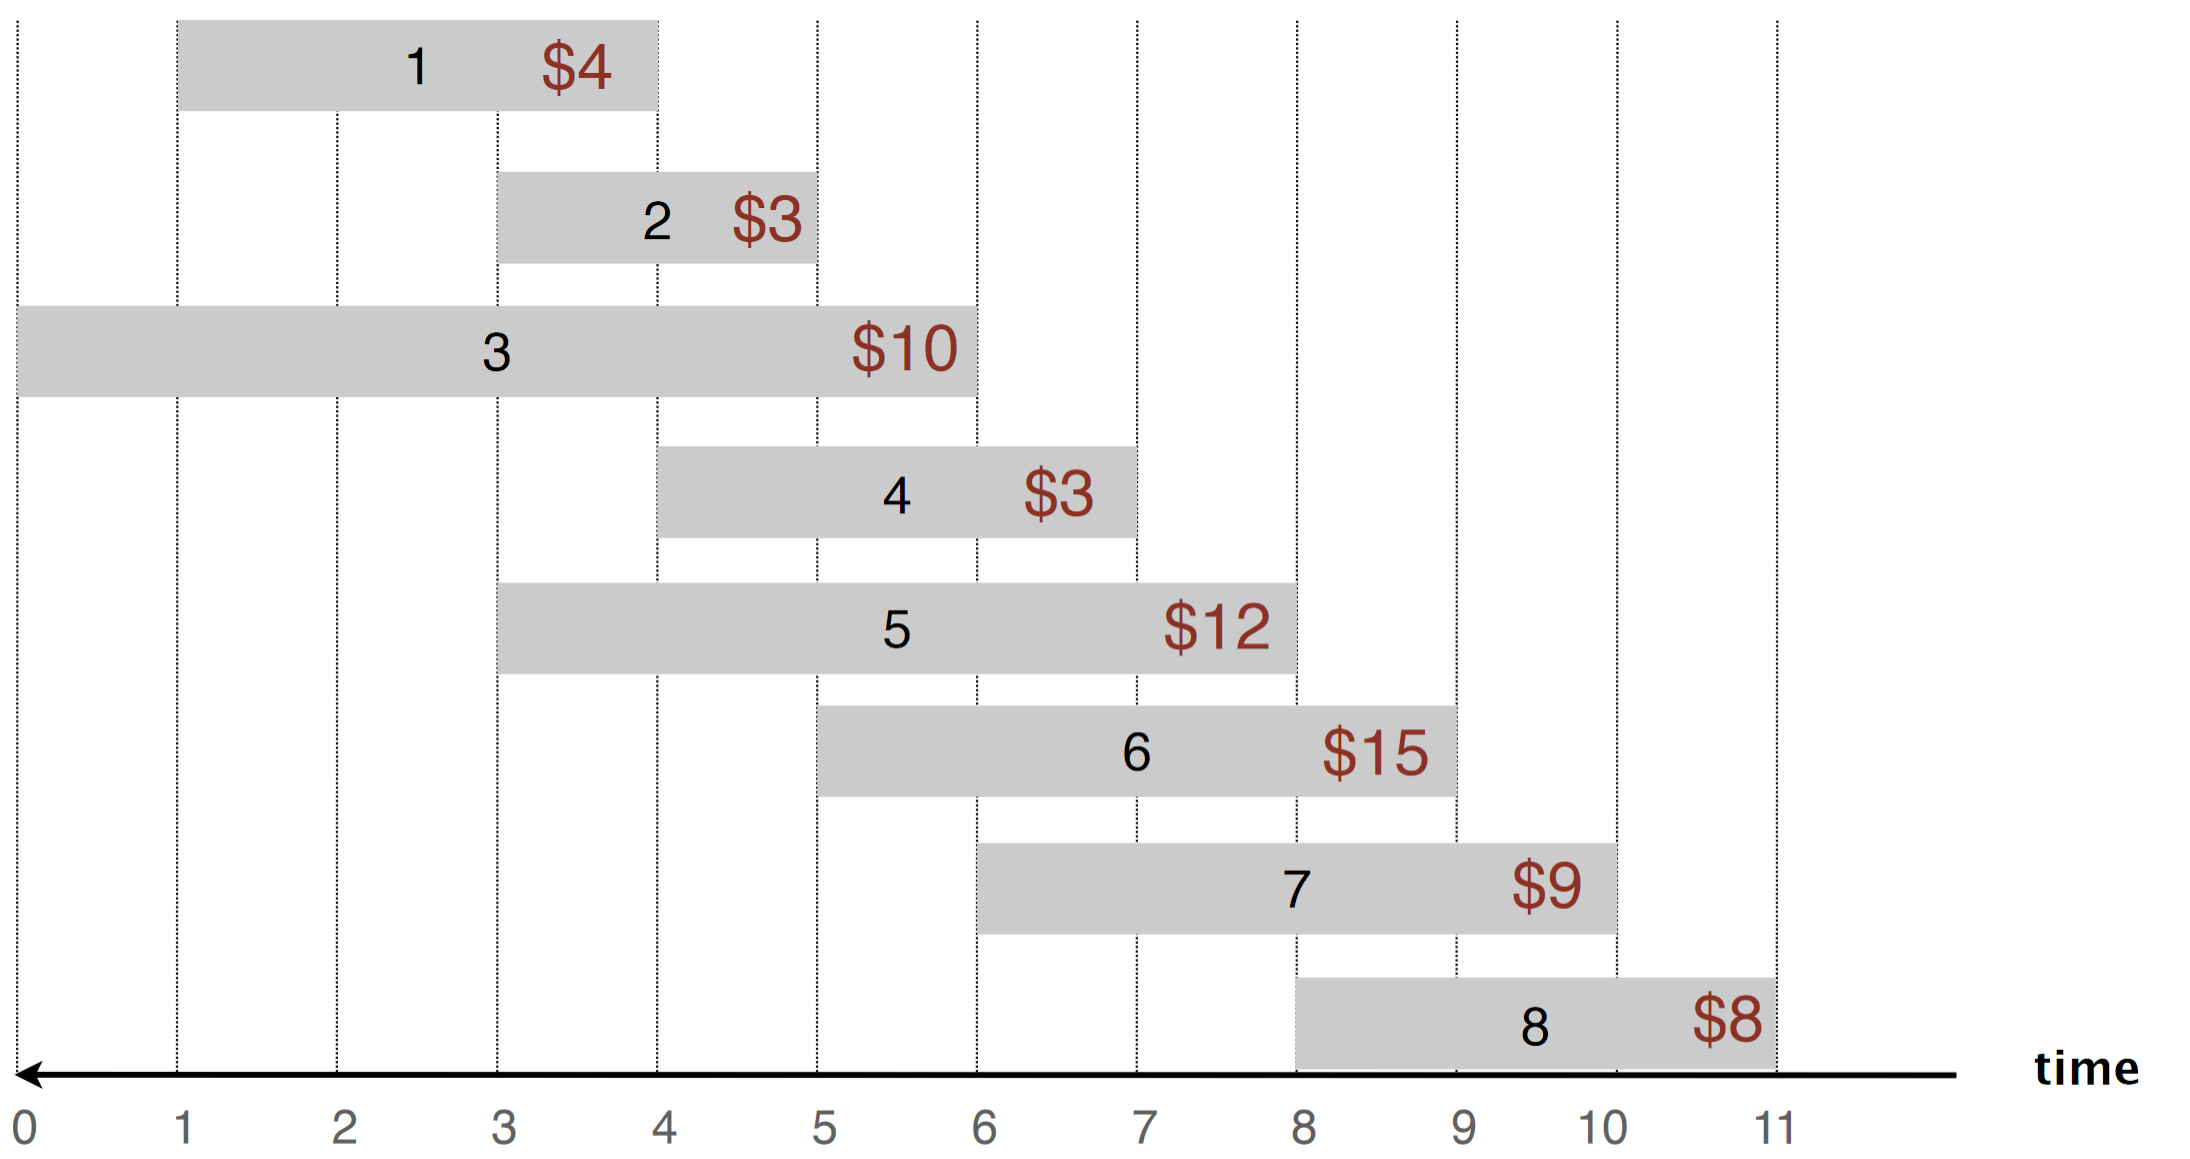
\includegraphics[width=.9\textwidth]{Sections/dp/b_wis.png}
    \caption{Optimal Values for Each Index $j$}
    \label{fig:wis}
\end{figure}

\vspace{-1em}
\noindent
Where,\\
$OTP[1]\gets max\{v_1+OPT(p(1)), OPT(0)\} = max\{4+0, 0\} = 4$;\\
$OPT[2]\gets max\{v_2+OPT(p(2)), OPT(1)\} = max\{4+0, 4\} = 4$;\\
$OPT[3]\gets max\{v_3+OPT(p(3)), OPT(2)\} = max\{10+0, 4\} = 10$;\\
$OPT[4]\gets max\{v_4+OPT(p(4)), OPT(3)\} = max\{3+4, 10\} = 10$;\\
$OPT[5]\gets max\{v_5+OPT(p(5)), OPT(4)\} = max\{12+0, 10\} = 12$;\\
and so on.

\newpage

\section{Backtracking}
\noindent

\begin{Def}[Backtracking]

    During recursion we may build solutions based on some number of constraints. During recursion, if 
    we at all, hit some constraint or \textit{dead-end}, we \textbf{backtrack} to a previous state to try another path.\\

    \noindent
    Additionally, after a solution is found, we may want to trace which calls lead to our solution. This also called \textbf{backtracking}.
\end{Def}

\noindent
Given our weighted interval scheduling (WIS) problem in Figure (\ref{fig:wis}), we want to reverse-engineer the jobs that gave us
our final solution. Since we have already computed all $OPT(j)$ stored in $OPT[\ ]$, and all $p(j)$, we can backtrack
to find the jobs that gave us our optimal solution.

\begin{Func}[Backtracking Weighted Interval Scheduling - \textit{Backtrack()}]
    \label{func:backtrack}
    \vspace{-.5em}
    \begin{algorithm}[H]
        \SetAlgoLined
        \SetKwProg{Fn}{Function}{:}{}
        \tcp{$OPT[\ ]$ (optimal solutions of $j$ job) and $p()$ (next comptible job) are already computed for $1,\dots,j$}
        $j \gets OPT.length-1$; $S \gets \{\}$; \tcp{$S$ is our set of jobs}
        $Backtrack(OPT, j)$\;
        \Fn{\textit{Backtrack}(OPT, j)}{

                \If{$v_j+OPT[p(j)] > OPT[j-1]$}{
                    \Return $S \cup Backtrack(OPT, p(j))$\;
                }
                \Else{
                    \Return $Backtrack(OTP, j-1)$\;
                }

        }
    \end{algorithm}
    \noindent
    \rule{\textwidth}{0.4pt}
    \textbf{Correctness:} In our example above, the WIS's last index was the optimal solution. However, let $8=\$1$, then
    jobs $(6,1)$ would have been the optimal solution. This leaves $OPT[8]=\$19$, rather than $\$20$. Line 4 finds the first occurance where
    we found the optimal solution. As if we first found the optimal solution at index $6$, then $6,\dots,j$ would contain $OPT(6)$. This is why
    we exclude the choice $(7,3)=\$19$.\\

    \noindent
    We then repeat such pattern on the next compatible job. We know the set $N:=\{1\dots p(j)\}$ must contain an element of the optimal solution.
    Similar to our Dijkstra's proof (\ref{fig:dstra_proof}), that within the optimal path, a subpath's shortest path is also optimal. We check if
    $p(j)$ is the first occurance of the optimal solution in $N$, if not we continue to backtrack.\\

    \noindent
    \textbf{Time Complexity:} $O(n)$. At most, iterate through all $n$ jobs, and add them to our set $S$.
\end{Func}
\noindent
\underline{Notice that our backtracking closely mimics our orginal recursive formula.}

\newpage
\section{Subset Sum}
\subsection{Weighted Ceiling}


\begin{Def}[Problem - Subset Sum (Weighted Ceiling)]

Given a set of integers, say $S=\{3,6,1,7,2\}$, and a target sum $T=9$, find the max subset $P$ of $S$, such that $P\leq T$.
\end{Def}

\noindent
We know that when building our solution, we may pick $S_i$ and try all other combinations with $S_{i+1},\dots,S_n$ where $n=|S|$.
This may cause us to repeat computations as we build our solution. We now know to use dynamic programming to store our results. We
start by finding subproblems:

\[
    S=\{3,6,1,7,2\}, T=9 \text{; (choose 3)$\Rightarrow$ } S'=\{6,1,7,2\}, T'=6
\]

\noindent
Where $S'$ and $T'$ are $S$ and $T$ after removing 3. If we kept $T=9$, then we'd be asking, ``find a max subset $P$ of $S'$, s.t., $P\leq 9$,'' which
isn't our goal. If we decide $3\in P$, then $S'$ may also contain an optimal contribution (similar to our above Proof (\ref{func:backtrack})). While
building our solution, if $S_i>T$ we know not to consider it.\\

\noindent
We derive the following cases, where $T$ is a changing target sum, and $S_i$ the value of index $i$  (Alternitevely we could use subtraction, instead popping tail elements rather than head elements):

\vspace{-1em}
\begin{align*}
    OPT(i, T) =
    \begin{cases}
        0 & \text{if $T=0$}\\
        OPT(i+1, T) & \text{if $S_i > T$}\\
        max\{\underbracket{OPT(i+1, T)}_{\text{next solution}}, \underbracket{S_i+OPT(i+1, T-S_i)}_{\text{build solution}}\} & \text{else}
    \end{cases}
\end{align*}
\noindent
Moreover, if $S_i$ is compatible with $T$, we check other solutions.
In WIS (\ref{sec:WIS}), we only kept track of one changing variable.
However, in this case, we change 2 states during each recurrence; 
Hence our array is two-dimensional:

\vspace{0em}
\begin{table}[h!]
    \centering
    \resizebox{\textwidth}{!}{%
    \begin{tabular}{c|cccccccccc}
    \toprule
    \rowcolor{OliveGreen!10} & \multicolumn{10}{c}{\textbf{Target Sum} \( t \)} \\
    \rowcolor{OliveGreen!10}
    \textbf{Index} \( i \) & 0 & 1 & 2 & 3 & 4 & 5 & 6 & 7 & 8 & 9 \\
    \midrule
    $\{\}$ & 0 & 0 & 0 & 0 & 0 & 0 & 0 & 0 & 0 & 0 \\
    4 (\{2\}) & 0 & 0 & 2 & 2 & 2 & 2 & 2 & 2 & 2 & 2 \\
    3 (\{7,2\}) & 0 & 0 & 2 & 2 & 2 & 2 & 2 & 7 & 7 & 9 \\
    2 (\{1,7,2\}) & 0 & 1 & 2 & 3 & 3 & 3 & 3 & 7 & 8 & 9 \\
    1 (\{6,1,7,2\}) & 0 & 1 & 2 & 3 & 3 & 3 & 6 & 7 & 8 & 9 \\
    0 (\{3,6,1,7,2\}) & 0 & 1 & 2 & 3 & 4 & 5 & 6 & 7 & 8 & 9 \\
    \bottomrule
    \end{tabular}
    }
    \caption{Subset Sum Dynamic Programming Table (DP Table), where $OTP[i][t]$ is the max combination $P$ of $S_i,\dots,S_n$ s.t., $P\leq t$.}
    \label{tab:subset}
    \end{table}

    \noindent
    \underline{An additional explanation of the above table on the next page.}

    \newpage

    \noindent
    The above table (\ref{tab:subset}), when we reach $i=4$, we only have $\{2\}$ to consider. This is fine as we've
    already considered all $2$'s possible combinations. Observe a nested for-loop approach to find all pairs in $S=\{3,6,1,7,2\}$:

    \begin{itemize}
        \item Start with 3, then: $\{(3,6),(3,1),(3,7),(3,2)\}$
        \item Then with 6, then: $\{(6,1),(6,7),(6,2)\}$
        \item Then with 1, then: $\{(1,7),(1,2)\}$
        \item Then with 7, then: $\{(7,2)\}$
        \item Then with 2, then: $\{2\}$
    \end{itemize}

    \noindent
    Notice how we already found all 2's combinations, $(3,2),(6,2),(1,2),(7,2)$. So even though we only have 2 to consider at $i=4$, we've
    already accounted for all possible combinations.\\

    \noindent
    Hence the algorithm below. We change the next and build step to subtraction to allow us to mimic recursion in a 
    bottom up approach. Here we start at the top left progressing forward, rather than the bottom right:
    \begin{Func}[Subset Sum - \textit{OPT()}]
        \label{func:subset}
        \vspace{-.5em}
        \begin{algorithm}[H]
            \SetAlgoLined
            \SetKwProg{Fn}{Function}{:}{}
            $S$; $T$; $OPT[\ ][\ ]$; \tcp{Set $S$, Weight cieling $T$, DP table $OPT(i, T)$}
            $OPT[0][*] \gets 0$; \tcp{Base case (array of size $0$)}
            $OPT[*][0] \gets 0$; \tcp{Base case (array of size $T=0$)}
            \For{$i \gets 1$ \KwTo $S.length$}{
                \For{$t \gets 1$ \KwTo $T$}{
                    
                    \If{$S[i] > t$}{
                        $OPT[i][t] \gets OPT[i-1][t]$\;
                    }
                    \Else{
                        $OPT[i][t] \gets max\{\underbracket{OPT[i-1][t]}_{\text{next solution}}, \underbracket{S[i]+OPT[i-1][t-S[i]]}_{\text{build solution}}\}$\;
                    }
                }
            }
            \textbf{return} $OPT$\;
        \end{algorithm}
        \noindent
        \rule{\textwidth}{0.4pt}
        \textbf{Time Complexity:} $O(nT)$. We iterate through all $n$ jobs, and for each job, we iterate through all $T$ target sums.
    \end{Func}

    \noindent
    The above table (\ref{tab:subset}) shows our best possible combination at $OPT[0][9]$; However, we don't know which elements
    contributed to our solution. We backtrack to find such elements on the next page.

    \newpage 

    \noindent
    In our table below, ignore the fact that the numbers come out nicely. Where $OPT[0][9]=9$, could have been $OPT[0][9]=8$, if we excluded 2 and 3 from our orginal set.\\

    \noindent
    We want to know at each stage, what $S_i$ we picked to obtain $T$. Just like, in our WIS problem (\ref{func:backtrack}), we want to know 
    the first occurance of the optimal solution existing. I.e., which $S_i$ was first to contribute to our solution.\\
    
    \noindent
    Below we give the algorithm to compute such, and an explanation below the table:
    

    \begin{Func}[Backtracking Subset Sum - \textit{Backtrack()}]

        \vspace{-.5em}
        \begin{algorithm}[H]
            \SetKwProg{Fn}{Function}{:}{}
            $i \gets 0$; $t \gets T$; $S \gets \{\}$; \tcp{$S$ is our set of jobs}
            $Backtrack(OPT, i, t)$\;
            \Fn{\textit{Backtrack}(OPT, i, t)}{
                \tcp{Where $OTP.length$ is the number of rows}
                \While{$i < OPT.length$}{
                    \If{$OPT[i][t] > OPT[i+1][t]$}{
                        $S \gets S \cup \{S[i]\}$\;
                        $t \gets t-S[i]$\;
                    }
                    $i \gets i+1$\;
                }
                \Return $S$\;
            }
        \end{algorithm}
        \noindent
        \rule{\textwidth}{0.4pt}
        \textbf{Time Complexity:} $O(n)$. At most, iterate through all $n$ jobs, and add them to our set $S$.
    \end{Func}

\vspace{-2em}
\begin{table}[h!]
    \centering
    \resizebox{\textwidth}{!}{%
    \begin{tabular}{c|cccccccccc}
    \toprule
    \rowcolor{OliveGreen!10} & \multicolumn{10}{c}{\textbf{Target Sum} \( t \)} \\
    \rowcolor{OliveGreen!10}
    \textbf{Index} \( i \) & 0 & 1 & 2 & 3 & 4 & 5 & 6 & 7 & 8 & 9 \\
    \midrule
   $\{\}$ & 0 & 0 & 0 & 0 & 0 & 0 & 0 & 0 & 0 & 0 \\
    4 (\{2\}) & 0 & 0 & \cellcolor{purple!10}2 & 2 & 2 & 2 & 2 & 2 & 2 & 2 \\
    3 (\{7,2\}) & 0 & 0 & 2 & 2 & 2 & 2 & 2 & 7 & 7 & \cellcolor{purple!10}9 \\
    2 (\{1,7,2\}) & 0 & 1 & 2 & 3 & 3 & 3 & 3 & 7 & 8 & 9 \\
    1 (\{6,1,7,2\}) & 0 & 1 & 2 & 3 & 3 & 3 & 6 & 7 & 8 & 9 \\
    0 (\{3,6,1,7,2\}) & 0 & 1 & 2 & 3 & 4 & 5 & 6 & 7 & 8 & 9 \\
    \bottomrule
    \end{tabular}

    }
    \end{table}

\noindent
Here we know 3 combinations did not start our solution, neither did 6 or 1. However, 7 combinations did.
We know that $7\in P$. We reduce $T$ to $2$, and our first element to contribute to the optimal solution was 2. 
We reduce again hitting $0$, hence, $P=\{7,2\}$.

\newpage
\subsection{Knapsack}

\begin{Def}[Problem - Subset Sum (Knapsack)]

    Given a set $S$ of $n$ items, each with a weight $w_i$ and value $v_i$, and a knapsack of capacity $W$, find a subset
    $P$ of $S$, s.t., $\sum_{i\in P}w_i\leq W$ and $\sum_{i\in P}v_i$ is the highest value achievable.
\end{Def}   

    \begin{minipage}{0.45\textwidth}

        To the right is an example of a knapsack instance. 
        Say we want to solve this by repeatedly taking some combination of weights and their totals.
        Each time we take an item, we can no longer choose it, and our knapsack weight and value increase.
        Our base case must be when we run out of items. We also know to step back when we exceed our weight limit.
        
        We want our build step to track the value in some way, decrement our choices, and decrease our weight limit. Then 
        if we don't pick the item, we move to the next item with no change in weight or value.
        This becomes strikingly similar to the previous subset sum problem with minor adjustments:

    \end{minipage}
    \begin{minipage}{0.45\textwidth}
        \begin{center}
            \begin{tabular}{|c|c|c|}
            \hline
            $i$ & $v_i$ & $w_i$ \\
            \hline
            1 & 1 & 1 \\
            2 & 6 & 2 \\
            3 & 18 & 5 \\
            4 & 22 & 6 \\
            5 & 28 & 7 \\
            \hline
            \end{tabular}
            
            \vspace{0.3cm}
            \textbf{knapsack instance} \\
            (weight limit $W = 11$)
        \end{center}
    \end{minipage}
    \begin{align*}
        OPT(i, w) =
        \begin{cases}
            0 & \text{if $i==0$}\\
            OPT(i-1, w) & \text{if $w_i > w$}\\
            max\{\underbracket{OPT(i-1, w)}_{\text{next solution}}, \underbracket{v_i+OPT(i-1, w-w_i)}_{\text{build solution}}\} & \text{else}
        \end{cases}
    \end{align*}
    \vspace{-1em}
    \begin{figure}[h]
       
        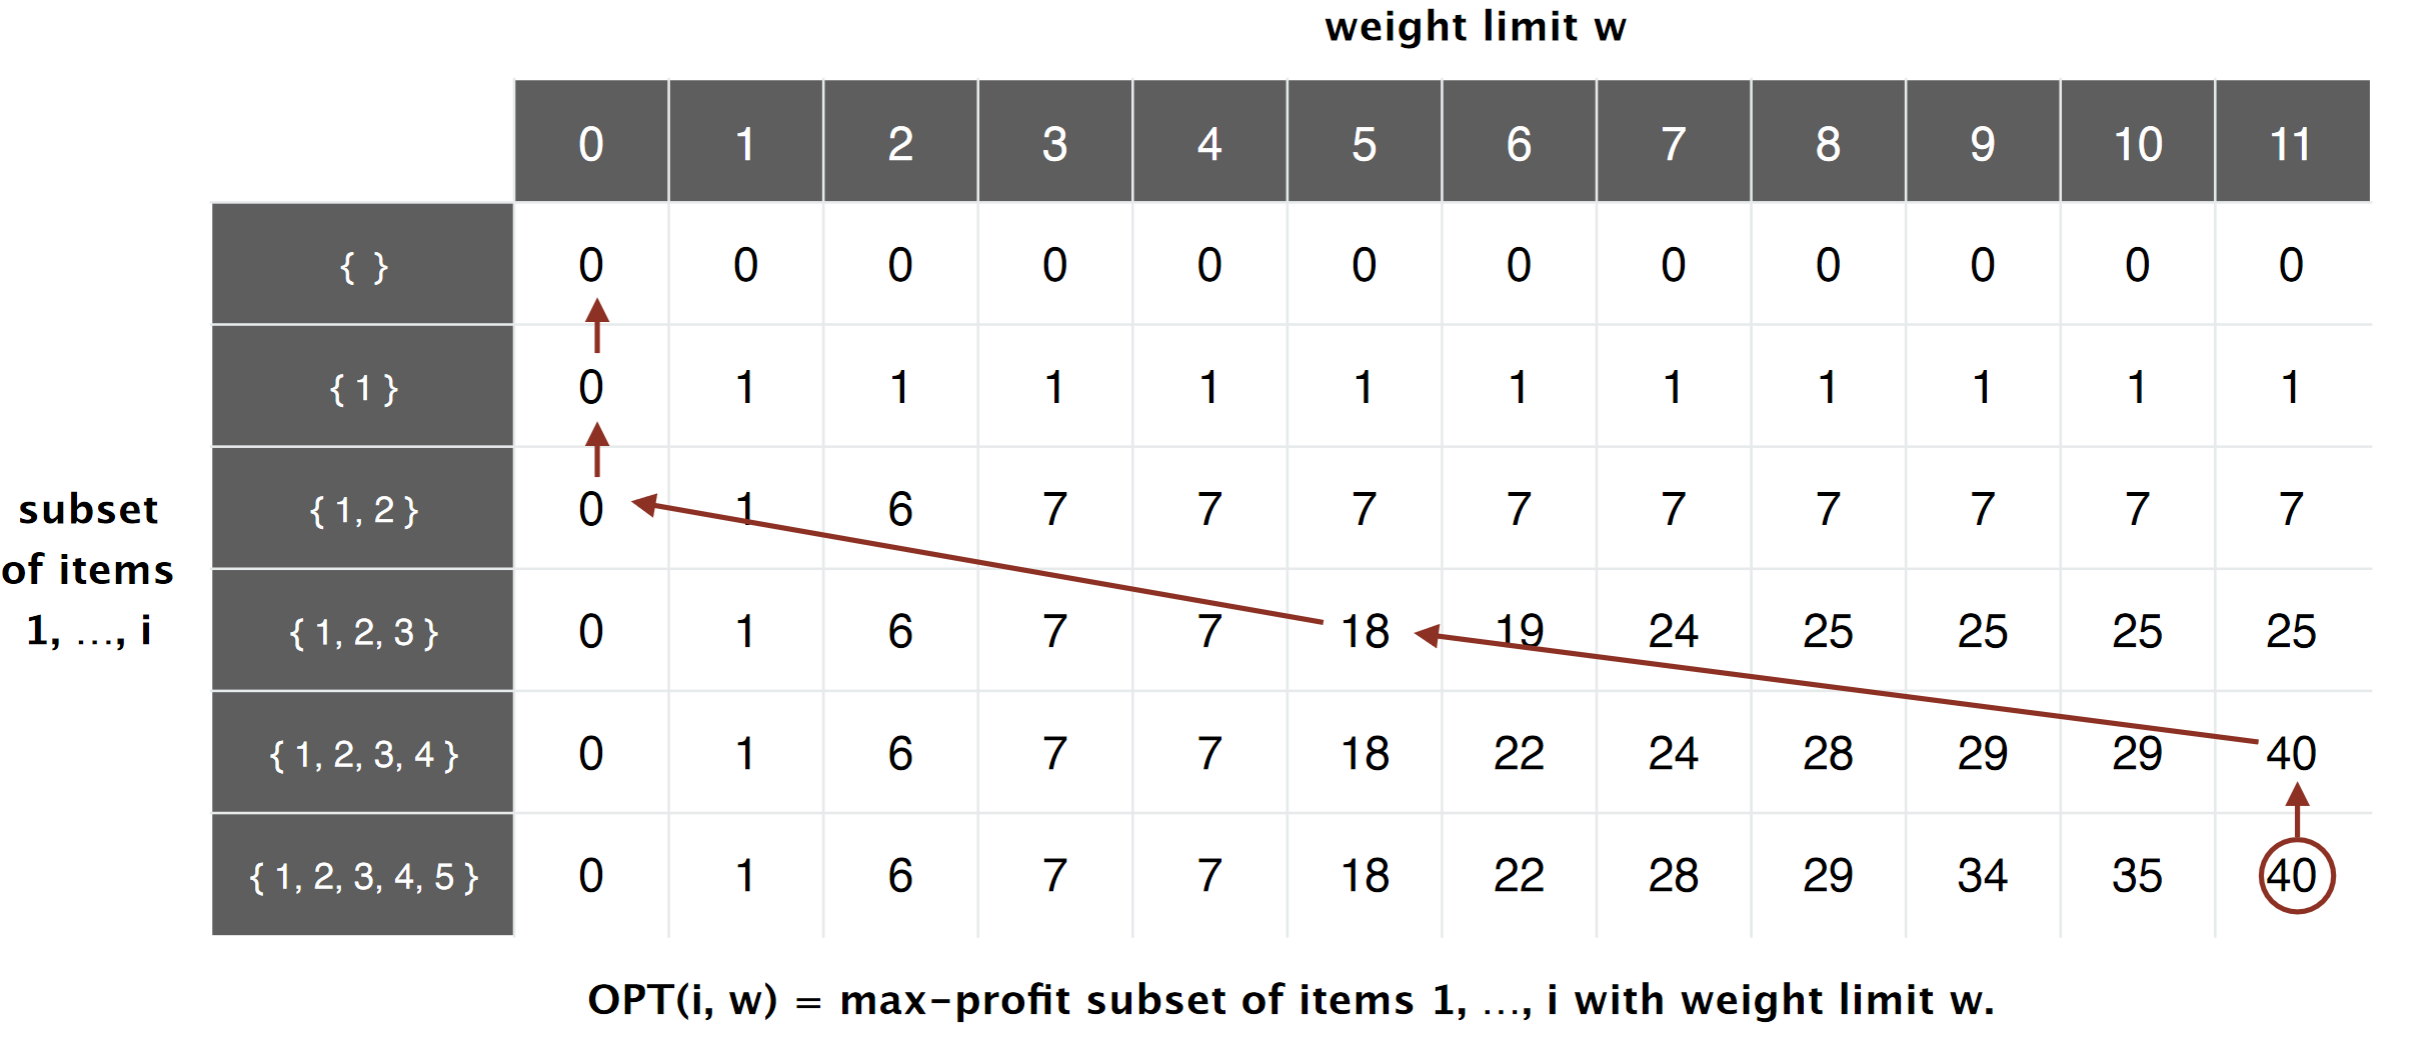
\includegraphics[width=.95\textwidth]{Sections/dp/knapsack.png}
    \end{figure}
    \label{fig:knapsack}

    \noindent
    We achieve the a similar table as we saw before in the subset sum problem.

    \newpage

    \noindent
    We skip the implementation as the function is the same as Function (\ref{func:subset}), with the only difference being that we add $v_i$ instead of $S_i$ at build step.
    Again the runtime is the dimension of our DP table, $O(nW)$.
    \begin{Func}[Backtracking Knapsack- \textit{Backtrack()}]
        \label{func:knapsack}

        \vspace{-.5em}
        \begin{algorithm}[H]
            \SetKwProg{Fn}{Function}{:}{}
            $i \gets OPT.length$; $w \gets W$; $S \gets \{\}$; \tcp{$S$ is our set of jobs}
            \While{$i > 0$ AND $w > 0$}{
                \If{$OPT[i][w] > OPT[i-1][w]$}{
                    $S \gets S \cup \{i\}$\;
                    $w \gets w-w_i$\;
                }
                $i \gets i-1$; \tcp{In both cases we $i-1$}
            }
            \Return $S$\;
            
        \end{algorithm}
        \noindent
        \rule{\textwidth}{0.4pt}
        \textbf{Time Complexity:} $O(n)$.
    \end{Func}

\subsection{Unbounded Knapsack}
\begin{Def}[Problem - Unbounded Knapsack]

    Given a set $S$ of $n$ items, each with a weight $w_i$ and value $v_i$, and a knapsack of capacity $W$, find a subset
    $P$ of $S$, s.t., $\sum_{i\in P}w_i\leq W$ and $\sum_{i\in P}v_i$ is the highest value achievable. There are 
    infinite copies of each item.
\end{Def}
\noindent
The same logic applies from the above knapsack problem. However, we can now take an item multiple times, meaning 
we may have to iterate over all possible choices between each item. We proceed as follows:

\begin{align*}
    OPT(i, w) =
    \begin{cases}
        0 & \text{if $i==0$}\\
        OPT(i-1, w) & \text{if $w_i > w$}\\
        {\displaystyle \max_{j = 0, \dots, \infty}}\{\underbracket{OPT(i-1, w)}_{\text{next solution}}, \underbracket{j\cdot v_i+OPT(i-1, w-j\cdot w_i)}_{\text{build solution}}\} & \text{else}
    \end{cases}
\end{align*}
At each build step we iterate $j\to\infty$, until $w_i\cdot j > w$. This third step may seem 3-dimensional, as in 
our $n\times W$ table, each entry has another $W$ entries. However, there's no need to store all $W$ entries, as we only 
need to store $j$.

Moreover, we don't want to directly store $j$ in our table $OPT$ as it would overwrite the $v_i$ value. 
Instead, we keep two tables both $n\times W$, so that we can read both values $v_i$ and its $j$.

\newpage

\noindent
Let us call our choices $j$ table $C$ and our value table $M$. We illustrate this relationship
by imagining the two tables sandwiched on top of each other. Then for every $i$ and $w$ we can reference both values at the same time:

\begin{figure}[h]
    \centering
    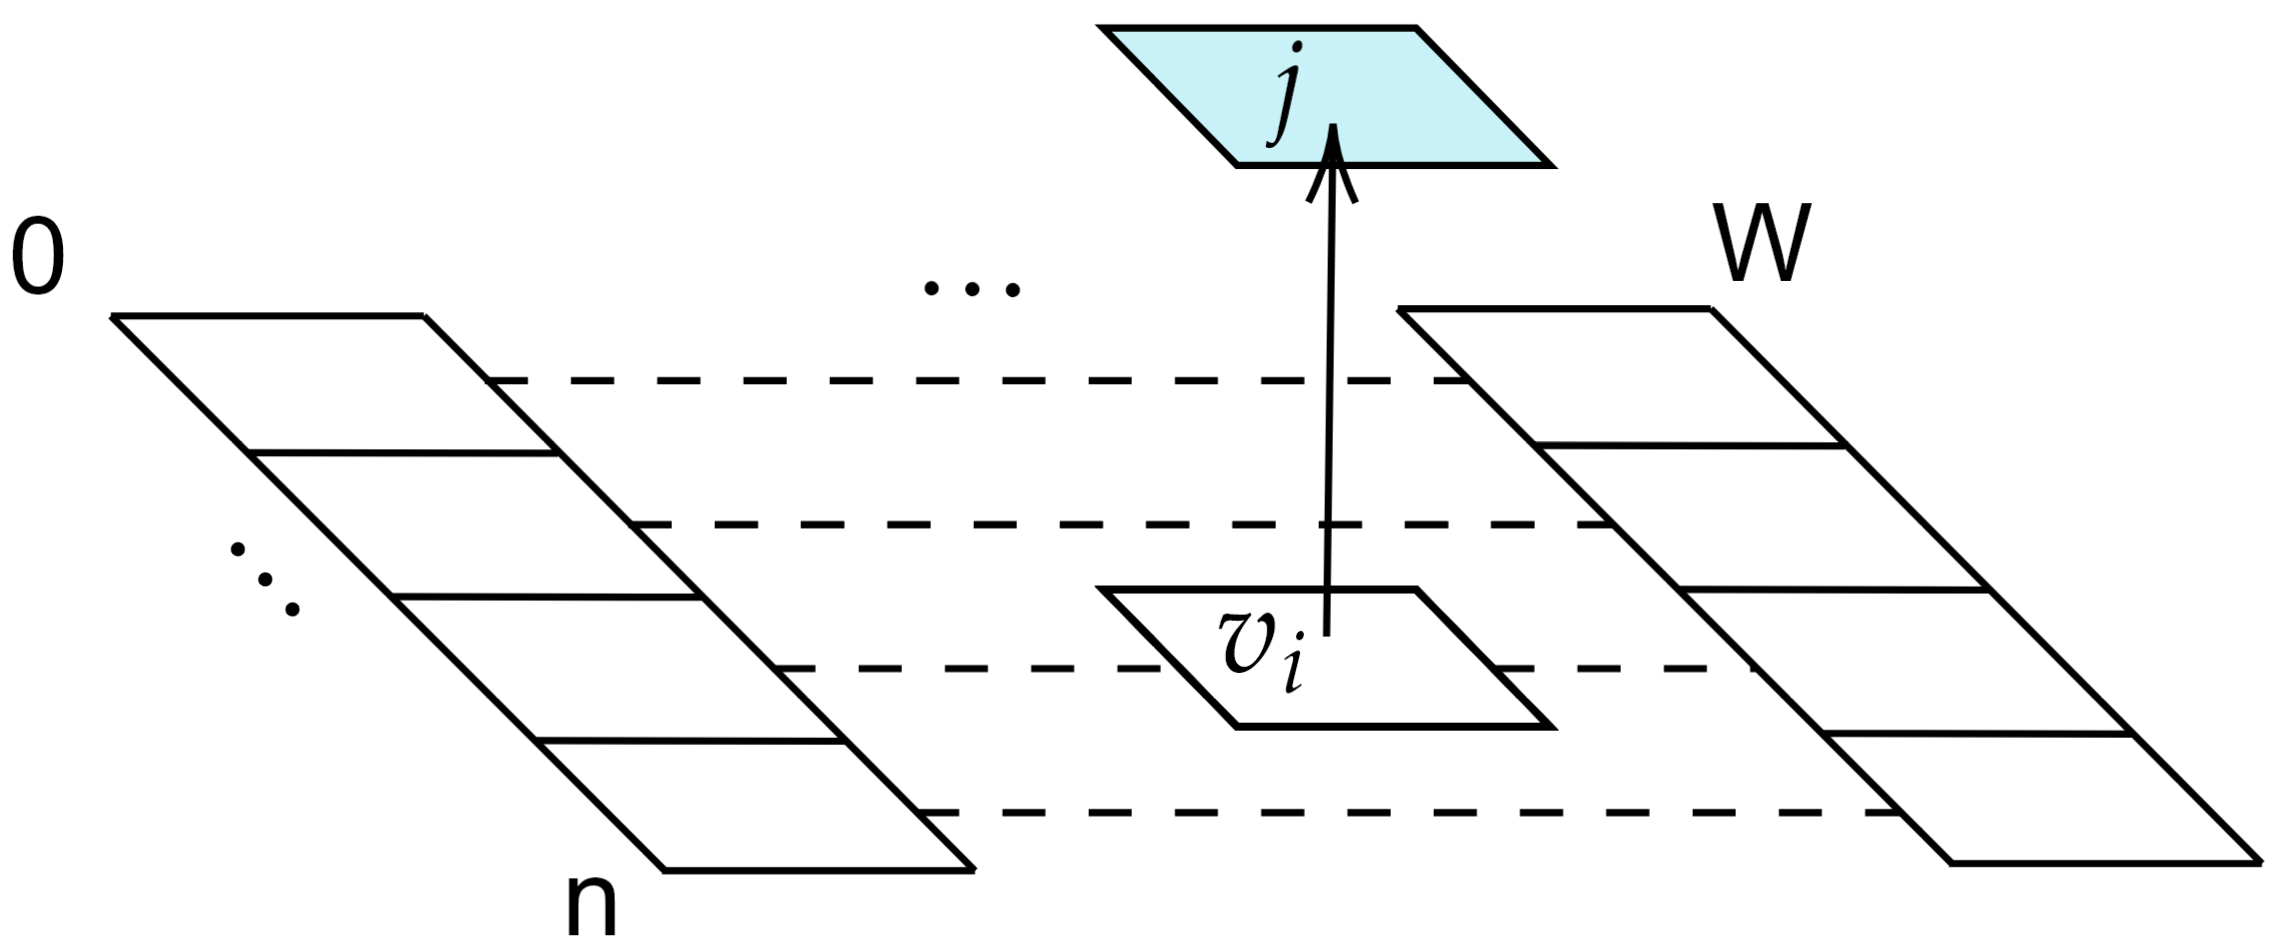
\includegraphics[width=.5\textwidth]{Sections/dp/sandwich.png}
    \caption{Illustrating the relationship between $C$ and $M$, where $v_i$ relates to its respective $j$} 
    
\end{figure}

\noindent
We implement the following algorithm:

\begin{Func}[Unbounded Knapsack - \textit{UnboundedKnapsack()}]

    \vspace{-.5em}
    \begin{algorithm}[H]
        \SetKwProg{Fn}{Function}{:}{}
        $M \gets (n+1) \times (W+1)$ table \tcp{DP table}
        $C \gets (n+1) \times (W+1)$ table \tcp{Number of copies}
        $M[0][*] \gets 0$ and $M[*][0] \gets 0$\;
        
        \For{$i \gets 1$ \KwTo $n$}{
            \For{$w \gets 1$ \KwTo $W$}{
                $M[i][w] \gets M[i-1][w]$; \tcp{Start with previous solution}
                $m \gets 1$\;
                
                \While{$m \cdot w_i \leq w$}{
                    $val \gets m \cdot v_i + M[i-1][w - m \cdot w_i]$\;
                    \If{$val > M[i][w]$}{
                        $M[i][w] \gets val$\;
                        $C[i][w] \gets m$\;
                    }
                    $m \gets m + 1$\;
                }
            }
        }
        \Return $M, C$\;
    \end{algorithm}
    
    \noindent
    \rule{\textwidth}{0.4pt}
    \textbf{Time Complexity:} $O(n \times W^2)$ Though we said our tables won't need to be $W$ deep, we still iterate at most $W$ times for each $w$.\\
    \textbf{Space Complexity:} $O(n \times W)$, as $M$ and $C$ are both $n \times W$, hence $nW+nW=O(nW)$.
\end{Func}

\newpage
\noindent
Our backtracking algorithm is almost identical to the previous knapsack problem (\ref{func:knapsack}), however, we now have to consider the number of copies $C[i][w]$.
\begin{Func}[Backtracking Unbounded Knapsack - \textit{BKBacktrack()}]

    \vspace{-.5em}
    \begin{algorithm}[H]
        \SetKwProg{Fn}{Function}{:}{}
        $sol \gets \emptyset$\;
        $i \gets n$ and $w \gets W$\;
        
        \While{$i > 0$ \textbf{and} $w > 0$}{
            $sol \gets sol \cup \{i \cdot C[i][w]\}$; \tcp{Add item $i$ with its count $C[i][w]$}
            $w \gets w - C[i][w] \cdot w_i$\;
            
            $i \gets i - 1$\;
        }
        
        \Return $sol$\;
    \end{algorithm}
    
    \noindent
    \rule{\textwidth}{0.4pt}
    \textbf{Time Complexity:} $O(n)$, just like before, as we traverse vertically up our $n\times W$ table, finding at what point $M[i][w]$ change. 
    This indicates $i$ was used in the solution.
\end{Func}
% \begin{Func}[Backtracking Unbounded Knapsack - \textit{BKBacktrack()}]

%     \vspace{-.5em}
%     \begin{algorithm}[H]
%         \SetKwProg{Fn}{Function}{:}{}
%         $sol \gets \emptyset$\;
%         $i \gets n$ and $w \gets W$\;
        
%         \While{$i > 0$ \textbf{and} $w > 0$}{
%             \If{$M[i][w] > M[i-1][w]$}{
%                 $sol \gets sol \cup \{(i, C[i][w])\}$; \tcp{Add item $i$ with its count $C[i][w]$}
%                 $w \gets w - C[i][w] \cdot w_i$\;
%             }
%             $i \gets i - 1$\;
%         }
        
%         \Return $sol$\;
%     \end{algorithm}
    
%     \noindent
%     \rule{\textwidth}{0.4pt}
%     \textbf{Time Complexity:} $O(n)$, just like before, as we traverse vertically up our $n\times W$ table, finding at what point $M[i][w]$ change. 
%     This indicates $i$ was used in the solution.
% \end{Func}


\subsection*{Unbounded knapsack (Bottom-Up Approach)}
\noindent
Alternatively we can use a bottom-up approach with a slight modification to our recursive formula. Instead of iterating over $j$, we iterate over $w$, 
continuously taking $v_j$ until we exceed $w$ or move onto the next item. This is shown by:
\[
\text{OPT}(i, w) = 
\begin{cases} 
    0 & \text{if } i = 0, \\
    \text{OPT}(i-1, w) & \text{if } w_i > w, \\
    \max\left(\text{OPT}(i-1, w), v_i + \text{OPT}(i, w - w_i)\right) & \text{otherwise.}
\end{cases}
\]

\noindent
Same scenerio, though now we build our solution $n\times W$ starting from the top left, rather than the bottom right. 
Meaning we start with one item, then two, then three, and so on.\\

\noindent
Each iteration we find the largest weight we can take as we grow our constraint $w$. While growing $w$ if the solution at 
at iteration $i$ is greater than the last, we take the item. This will consider all possible combinations.\\

\noindent
For an exercise, consider the previous table (\ref{fig:knapsack}), and follow the table left to right, top to bottom.

\newpage
\begin{Func}[Unbounded Knapsack - \textit{UnboundedKnapsack2()}]

    \vspace{-.5em}
    \begin{algorithm}[H]
        \SetKwProg{Fn}{Function}{:}{}
        $M \gets (n+1) \times (W+1)$ table$^*$ \tcp{DP table}
        $M[0][*] \gets 0$ and $M[*][0] \gets 0$ \tcp{Set first row and column to 0}
        
        \For{$i \gets 1$ \KwTo $n$}{
            \For{$w \gets 1$ \KwTo $W$}{
                \If{$w_i > w$}{
                    $M[i][w] \gets M[i-1][w]$;
                }
                \Else{
                    $val \gets v_i + M[i][w - w_i]$ \tcp{Take one more copy of $i$}
                    \If{$val > M[i-1][w]$}{
                        $M[i][w] \gets val$;
                    }
                    \Else{
                        $M[i][w] \gets M[i-1][w]$;
                    }
                }
            }
        }
        \Return $M$\;
    \end{algorithm}
    
    \noindent
    \rule{\textwidth}{0.4pt}
    \textbf{Time Complexity:} $O(n \times W)$, as we iterate over each item and weight once.
\end{Func}

\begin{Func}[Traceback Solution for Unbounded Knapsack - \textit{Traceback()}]

    \vspace{-.5em}
    \begin{algorithm}[H]
        \SetKwProg{Fn}{Function}{:}{}
        $i \gets n$ \tcp{Start from the last item}
        $w \gets W$ \tcp{Start from the maximum weight}
        $sol \gets \emptyset$ \tcp{Initialize the solution set}
        
        \While{$i > 0$ \textbf{and} $w > 0$}{
            \If{$w \geq w_i$ \textbf{and} $(v_i + M[i][w - w_i] > M[i-1][w])$}{
                $sol.\textit{add}(i)$ \tcp{Add item $i$ to the solution}
                $w \gets w - w_i$ \tcp{Reduce the weight}
            }
            \Else{
                $i \gets i - 1$ \tcp{Move to the previous item}
            }
        }
        \Return $sol$\;
    \end{algorithm}
    
    \noindent
    \rule{\textwidth}{0.4pt}
    \textbf{Time Complexity:} $O(n + W)$, as we traverse the DP table in reverse order.
\end{Func}













